\documentclass{article}
\usepackage{include/nips15submit_e,times}
\usepackage{hyperref}
\usepackage{url}
\usepackage[noend]{algpseudocode}
\renewcommand\algorithmicthen{}
\renewcommand\algorithmicdo{}
\usepackage{algorithm}
\usepackage{natbib}
\usepackage{graphicx}
\usepackage{array,booktabs}

\definecolor{mydarkblue}{rgb}{0,0.08,0.45}
\definecolor{myfavblue}{rgb}{0.1176, 0.392, 1.0}
\hypersetup{
    colorlinks=true,
    linkcolor=mydarkblue,
    citecolor=mydarkblue,
    filecolor=mydarkblue,
    urlcolor=mydarkblue}

\newcommand{\vw}{\mathbf{w}}
\newcommand{\vx}{\mathbf{x}}
\newcommand{\vy}{\mathbf{y}}
\newcommand{\vv}{\mathbf{v}}
\newcommand{\vf}{\mathbf{f}}
\newcommand{\vg}{\mathbf{g}}
\newcommand{\vi}{\mathbf{i}}
\newcommand{\vr}{\mathbf{r}}
\newcommand{\vzero}{\mathbf{0}}
\newcommand{\ones}[1]{\mat{1}_{#1}}
\newcommand{\eye}[1]{\mat{E}_{#1}}
\newcommand{\tra}{^{\mathsf{T}}}
\newcommand{\vect}[1]{{\bf{#1}}}
\newcommand{\mat}[1]{\mathbf{#1}}
\newcommand{\pderiv}[2]{\frac{\partial #1}{\partial #2}}
\newcommand{\npderiv}[2]{\nicefrac{\partial #1}{\partial #2}}

\title{Neural Molecular Fingerprints}

\author{
David Duvenaud\\
Harvard University\\
\texttt{dduvenaud@seas.harvard.edu}
\And
Dougal Maclaurin\\
Harvard University\\
\texttt{maclaurin@physics.harvard.edu}
\And
Ryan P. Adams\\
Harvard University\\
\texttt{rpa@seas.harvard.edu}
}

%\nipsfinalcopy % Uncomment for camera-ready version
\begin{document}
\maketitle

\begin{abstract}
Predicting properties of molecules requires functions that take graphs as inputs.
Molecular graphs are usually processed using off-the-shelf hash-based functions to produce fixed-size fingerprint vectors, which are then fed into standard machine learning methods.
We introduce a generalization of commonly-used molecular fingerprints based on convolutional neural networks which allows learning the entire feature pipeline.
We show that these data-driven features are more interpretable, and have better predictive performance on a variety of tasks.
\end{abstract}

\section{Introduction}
Recent work in materials design has applied deep learning to virtual screening, where the task is to predict the properties of novel molecules by generalizing from examples.
One difficulty with this task is that the input to the predictor, a molecule, can be of arbitrary size and shape.
Most machine learning pipelines can only handle inputs of a fixed size.
The current state of the art is to use off-the-shelf fingerprint software to compute fixed-dimensional feature vectors, and use those features as inputs to fully-connected deep neural networks or other standard machine learning methods.
This formula was followed by \citet{unterthinerdeep}, \citet{dahl2014multi}, and \citet{ramsundar2015massively}.
During training, the molecular fingerprints were treated as fixed.

In this paper, we replace the bottom layer of this stack -- the fixed molecular fingerprints -- with a differentiable neural network whose input is a graph representing the original molecule.
In this graph, vertices represent individual atoms and edges represent bonds.
The lower layers of this network is convolutional in the sense that the same local filter is applied to each atom and its neighborhood.
After several such layers, a global pooling step combines features from all the atoms in the molecule.
Figure \ref{fig:architecture sketch} shows a sketch of the network architecture.

Neural fingerprints offer several advantages over fixed fingerprints:
\begin{itemize}
\item {\bf Predictive performance.}
By using data adapting to the task at hand, machine-optimized fingerprints can provide substantially better predictive performance than fixed fingerprints.
We compare the effectiveness of neural fingerprints against standard fingerprints at predicting toxicity, solubility, drug efficacy, and organic photovoltaic efficiency.
\item {\bf Parsimony.}
Fixed fingerprints must be extremely large to encode all possible substructures without overlap.
For example, \cite{unterthinerdeep} used a fingerprint vector of size 43,000, after having removed rarely-occurring features.
Differentiable fingerprints can be optimized to encode only relevant features, reducing downstream computation and regularization requirements.
%In our tests, hyperparameter optimization usually chose fingerprint lengths of 20-50 for neural fingerprints, and near the maximum length (2048) for fixed fingerprints.
\item {\bf Interpretability.}
Standard fingerprints encode each fragment differently (up to random collisions), with no notion of similarity between fragments.
Each feature of a neural fingerprint can be activated by similar but distinct molecular fragments, making the feature representation more meaningful.
\end{itemize}

\begin{figure}
\centerline{\includegraphics[width=0.35\textwidth, clip, trim=4mm 12mm 4mm 4mm]{../../DeepMoleculesData/experiments/2015-06-01-fig1/1/fingerprint_computation_schematic.pdf}
\hspace{2em}
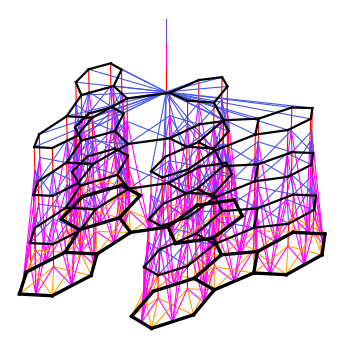
\includegraphics[width=0.4\textwidth, clip, trim=4mm 4mm 4mm 8mm]{figures/3d-nets/net1}}
\caption{\emph{Left}: A visual representation of the computational graph of both standard circular fingerprints and neural fingerprints.
First, at bottom, a graph is constructed matching the topology of the molecule being fingerprinted, in which edges represent bonds.
At each layer, information flows between neighbors in the graph.
Finally, each node in the graph turns on one bit in the fixed-length fingerprint vector.
This is a simplified sketch -- in reality, each layer writes to the fingerprint.
\emph{Right}: A more detailed graph also including the bond information used in each operation.}
\label{fig:architecture sketch}
\end{figure}

\section{Circular fingerprints}
The state of the art in molecular fingerprints are extended-connectivity circular fingerprints (ECFP)~\citep{ECFP2010}.
Circular fingerprints~\citep{glem2006circular} are a refinement of the Morgan algorithm~\citep{morgan1965generation}, designed to identify which substructures are present in a molecule in a way that is invariant to atom-relabeling.

Circular fingerprints generate each layer's features by applying a fixed hash function to the concatenated features of the neighborhood in the previous layer.
The results of these hashes are then treated as integer indices, where a 1 is written to the fingerprint vector at the index given by the feature vector at each node in the graph.
Ignoring collisions, each index of the fingerprint denotes the presence of a particular substructure.
The size of the substructures represented by each index depends on the depth of the network.
Thus the number of layers is referred to as the `radius' of the fingerprints.

%Our neural fingerprints could reasonably be said to generalize existing fingerprints.
%In Section \ref{sec:random is equivalent}, we show that randomly-initialized neural fingerprints have similar performance to existing fingerprints.

Circular fingerprints are analogous to convolutional networks in that they apply the same operation locally everywhere,  and combine information in a global pooling step.
%We believe the connection is not obvious and was not remarked upon before this paper.

\section{Creating a differentiable fingerprint}
The space of possible network architectures is large.
In the spirit of starting from a known-good configuration, we choose an architecture closely analogous to existing fingerprints.
This section describes our replacement of each discrete operation in circular fingerprints with a differentiable analog.

\paragraph{Hashing}
The purpose of the hashing function applied at each layer of circular fingerprints is to combine information about an atom and its neighboring substructures.
This ensures that any change in a fragment, no matter how small, will lead to a different fingerprint index being activated.
We replace this hash operation with a single layer of a neural network.
%, mapping from the concatenation of the features of an atom and its neighbors to a new feature vector for that atom.
This function is differentiable, and allows the computed result to be similar if the local molecular structure varies in small ways.

\paragraph{Indexing}
Circular fingerprints use an indexing operation to combine each atom's feature vector into a fingerprint.
Each atom sets a single bit of the fingerprint to one, at an index determined by the hash of its feature vector.
This pooling operation converts an arbitrary-sized graph into a fixed-sized vector.
For small molecules and a large fingerprint length, the fingerprints are always sparse.
We use the \texttt{softmax} operation as a differentiable analog of indexing.
In essence, each atom is asked to classify itself as belonging to a single category.
The sum of all these classification label vectors produces the final fingerprint.
%Each fingerprint has a specific meaning - arbitrary rotations of the weight matrices will not give rise to equivalent models.
This operation is analogous to the pooling operation in standard convolutional neural networks.
%For both circular and neural fingerprints, the fingerprint vector is written to at each layer.

\paragraph{Canonicalization}
Circular fingerprints are identical regardless of the ordering of atoms in each neighborhood.
This invariance is achieved by sorting the neighboring atoms according to their features, and bond features.
We experimented with this sorting scheme, and also with applying the local feature transform on all possible permutation of the local neighborhood.
An alternative to canonicalization is to apply a permutation-invariant function, such as summation.
In the interests of simplicity and scalability, we chose the summation.
%In some cases, this second approach requires more layers to distinguish

Algorithms \ref{alg:ecfp} and \ref{alg:neural} summarize these two algorithms and highlight their differences.
The parameters of neural fingerprints consist of a separate output weight matrix for each layer, as well as set of hidden-to-hidden weight matrices at each layer, one for each possible degree (up to 5).

\begin{figure*}[t]
 \begin{minipage}[t]{0.49\columnwidth}
 \begin{algorithm}[H]
\caption{Circular fingerprints} 
\label{alg:ecfp} 
\begin{algorithmic}[1]
\State \textbf{Input:} {molecule, radius $R$, fingerprint length $S$}
\State \textbf{Initialize:} {fingerprint vector $\vf \leftarrow \vzero_S$}
\For {each atom $a$ in molecule} 
    \State $\vr_a \leftarrow g(a)$ \Comment {lookup atom features}
\EndFor
\For {$L = 1$ to $R$} \Comment {for each layer}
	\For {each atom $a$ in molecule}
		\State $\vr_{1} \dots \vr_{N} = \textnormal{neighbors}(a)$
		\State $\vv \leftarrow [\vr_a \vr_{1} \dots, \vr_{N}]$ \Comment {concatenate}
		\State $\vr_a \leftarrow \textnormal{hash}(\vv)$ \Comment {hash function}
		\State $i \leftarrow \textnormal{mod}(r_a, S)$ \Comment {convert to index}		
		\State $\vf_{i} \leftarrow 1$ \Comment {Write 1 at index}
	\EndFor
\EndFor
\State \textbf{Return:} {binary vector $\vf$}
\end{algorithmic}
\end{algorithm}
\end{minipage}
\hfill
\begin{minipage}[t]{0.49\columnwidth}
\begin{algorithm}[H]
\caption{Neural fingerprints} 
\label{alg:neural} 
\begin{algorithmic}[1]
\State \textbf{Input:} {molecule, radius $R$, {\color{myfavblue} hidden weights $H_1 \dots H_R$, output weights $W_1 \dots W_R$}}
\State \textbf{Initialize:} {fingerprint vector $\vf \leftarrow \vzero_S$}
\For {each atom $a$ in molecule} 
	\State $\vr_a \leftarrow g(a)$ \Comment {lookup atom features}
\EndFor
\For {$L = 1$ to $R$} \Comment {for each layer}
    \For {each atom $a$ in molecule}
		\State $\vr_{1} \dots \vr_{N} = \textnormal{neighbors}(a)$
		\State $\vv \leftarrow [\vr_a \vr_{1}, \dots \vr_{N}]$ \Comment {concatenate}
		%\State $\vr_a \leftarrow {\color{myfavblue} \vf_{\theta_L}}(v)$ \Comment {{\color{myfavblue} smooth function}}
		\State $\vr_a \leftarrow {\color{myfavblue} \sigma(H_L \times \vv)}$ \Comment {{\color{myfavblue} smooth function}}
		\State $\vi \leftarrow {\color{myfavblue} \textnormal{softmax}(W_L \times \vr_a)}$ \Comment {{\color{myfavblue} sparsify}}
		\State $\vf \leftarrow {\color{myfavblue} \vf + \vi}$ \Comment {{\color{myfavblue}add to fingerprint}}
    \EndFor
\EndFor
\State \textbf{Return:} { {\color{myfavblue} real-valued} vector $\vf$}
\end{algorithmic}
\end{algorithm}
\end{minipage}
\hfill
\caption{Pseudocode of circular fingerprints (\emph{left}) and neural fingerprints (\emph{right}).
Differences are highlighted in blue.
Every non-differentiable operation is replaced with a differentiable analog.}
\end{figure*}


\section{Experiments}
\label{sec:experiments}

%\subsection{Randomly initialized neural fingerprints are similar to circular fingerprints}
\label{sec:random is equivalent}
Circular fingerprints can be interpreted as a special case of neural fingerprints having large random weights.
%To demonstrate that neural fingerprints are a generalization of circular fingerprints, in this section we give evidence that circular fingerprints are similar to neural fingerprints having large, randomly-initialized parameter vectors.
This is reasonable to expect, since in the limit of large input weights, \texttt{tanh} nonlinearities approach step functions, which when concatenated resemble a hash function.
Also, in the limit of large input weights, the \texttt{softmax} operator approaches a one-hot-coded \texttt{argmax} operator, which is analogous to an indexing operation.

\begin{figure}[h]
\centerline{\includegraphics[width=0.48\textwidth]{../../DeepMoleculesData/experiments/2015-05-04-compare-fingerprints/91-try-again/morg_conv_corr.pdf}
\includegraphics[width=0.5\textwidth]{../../DeepMoleculesData/experiments/2015-05-25-delaney/43-random-vs-depth/figures/all_rmsestest_rmse.pdf}}
\caption{\emph{Left:} Similarity between circular fingerprints and neural fingerprints with large random weights.
\emph{Right}: Predictive performance of circular fingerprints (red), neural fingerprints with fixed large random weights (green) and neural fingerprints with fixed small random weights (blue).
The performance of the large random weights is similar to that of circular fingerprints.}
\label{fig:fingerprint similarity}
\end{figure}

One use for molecular fingerprints is to compute distances between molecules.
We examined how similar inter-molecular distances were between ECFPs and neural fingerprints.
Figure~\ref{fig:fingerprint similarity} (left) shows a scatterplot of the similarity between fingerprints of circular and neural fingerprints of length 2048 on the \citet{delaney_data_2004} solubility dataset.
Similarity was measured using a continuous generalization of the Tanimoto (a.k.a.\ Jacard) similarity measure, given by
\begin{equation}
\textnormal{similarity}(\vx, \vy) =  \sum \min(x_i, y_i) \Big/ \sum \max(x_i, y_i)
\end{equation}
There is a correlation of $r = 0.823$ between the distances.
The line of points on the far left shows that for some pairs of molecules, binary ECFP fingerprints have exactly zero overlap.

Figure~\ref{fig:fingerprint similarity} (right) shows that the predictive performance of random neural fingerprints is similar to that of circular fingerprints.
Shown are average predictive performance on the same dataset using linear regression on top of fingerprints.
Both curves follow a similar trajectory, suggesting that randomly initialized neural fingerprints are similar to circular fingerprints.
In contrast, the performance of neural fingerprints with small random weights follows a different curve, and is substantially better.
This suggests the possibility that even for untrained neural weights, their relatively smooth activation helps generalization.

\subsection{Examining learned features}
To demonstrate that neural fingerprints are interpretable, we show examples of classes of substructures which activate individual features in a fingerprint.
Circular fingerprint features can each only be activated by a single fragment of a single radius, except for cases where different fragments randomly activate the same feature.
In contrast, neural fingerprints can be activated by variations of the same structure, making them more parsimonious and interpretable.

\paragraph{Solubility features}
%
\newcommand{\molfeature}[2]{\includegraphics[width=3.3cm, clip, trim = 2mm 3mm 2mm 3mm]{../../DeepMoleculesData/experiments/2015-05-30-visualize-fps/1/figures/fp_#1_highlight_#2.pdf}}%
\begin{figure}[h]%
\vspace{-2em}
\begin{tabular}{>{\centering}m{1.1in} >{\centering}m{3.1cm} >{\centering}m{3.1cm} >{\centering\arraybackslash}m{3.1cm}}
Fragments most activated by pro-solubility feature & \molfeature{15}{0} & \molfeature{15}{3} & \molfeature{15}{2} \\
\midrule
Fragments most activated by anti-solubility feature & \molfeature{18}{4} & \molfeature{18}{1} & \molfeature{18}{2}
\end{tabular}
\vspace{-3mm}
\caption{Examining fingerprints optimized for predicting solubility.
Shown here are representative samples of molecular fragments (highlighted in blue) which most activate different features of the  fingerprint.
\emph{Top row:} The feature having the strongest predictive weight for solubility.
\emph{Bottom row:} The feature having the strongest predictive weight against solubility.
%In contrast to circular fingerprints, which can each only be activated by a single fragment of a single radius, neural fingerprints can be activated by variations of the same structure, making them more parsimonious and interpretable.
}
\label{fig:learned features solubility}
\end{figure}
%
Figure \ref{fig:learned features solubility} shows fragments from the training set which maximally activated different features indices.
These fingerprints were trained to act as inputs to a linear model predicting the solubility as measured in the\citep{delaney_data_2004} dataset.
Shown are the two fingerprints with the strongest predictive weights.
The first fingerprint has a positive predictive relationship with solubility, and is most activated by fragments containing an OH group.
The second fingerprint, which is strongly negatively predictive of solubility, is activated by non-polar repeated ring structures.

\paragraph{Toxicity features}
We ran a similar experiment on datasets from the \citet{tox21}.
Figure \ref{fig:learned features toxicity} shows which fragments maximally activate various features.
%\newcommand{\molfeaturetox}[1]{\includegraphics[width=3.5cm]{figures/jorge-figures/#1.png}}%
\newcommand{\molfeaturetox}[2]{\includegraphics[width=3.4cm, clip, trim = 1mm 3mm 1mm 3mm]{../../DeepMoleculesData/experiments/2015-05-30-visualize-fps/5-toxic-diff-dataset/figures/fp_#1_highlight_#2.pdf}}%
\begin{figure}[h]
\begin{tabular}{>{\centering}m{1in} >{\centering}m{3.1cm} >{\centering}m{3.3cm} >{\centering\arraybackslash}m{3.1cm}}
Fragments most activated by toxicity feature on SR-MMP dataset
& 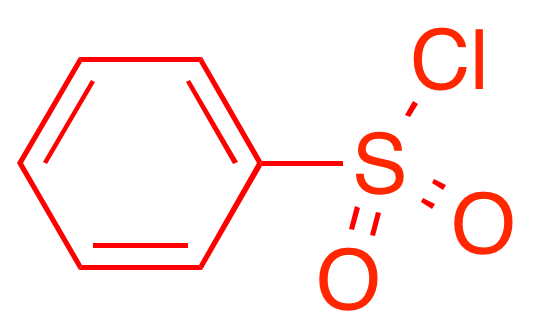
\includegraphics[width=2.2cm]{figures/jorge-figures/7.png} 
& 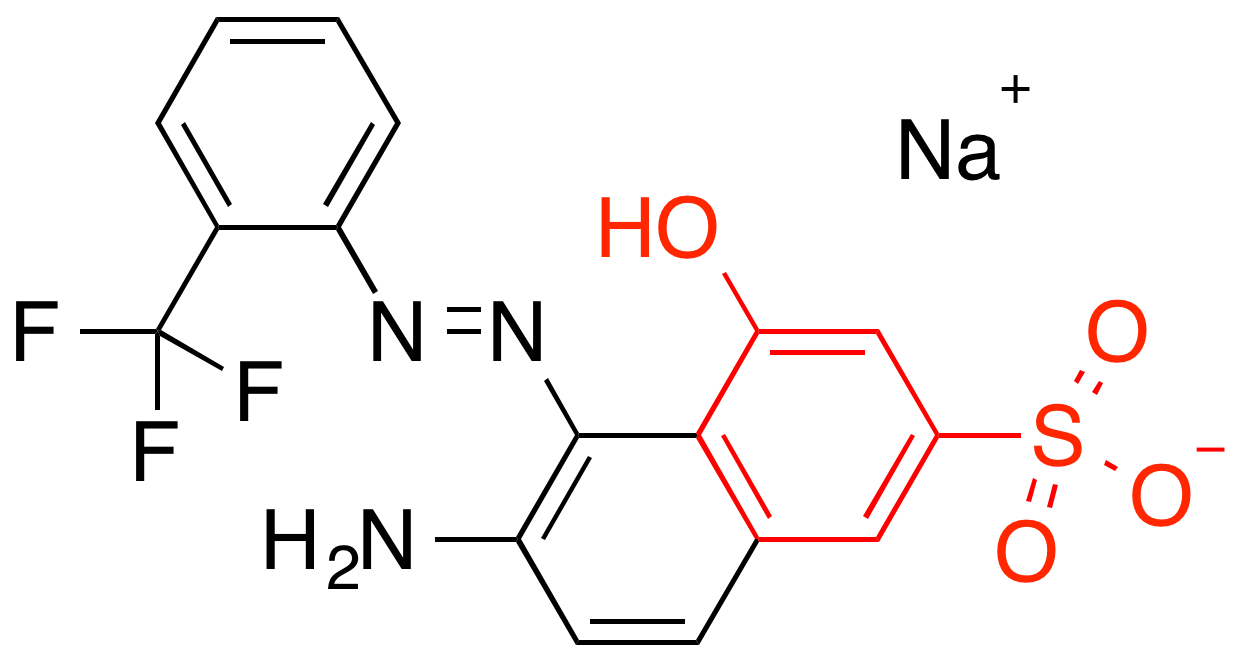
\includegraphics[width=3.3cm]{figures/jorge-figures/8.png}
& 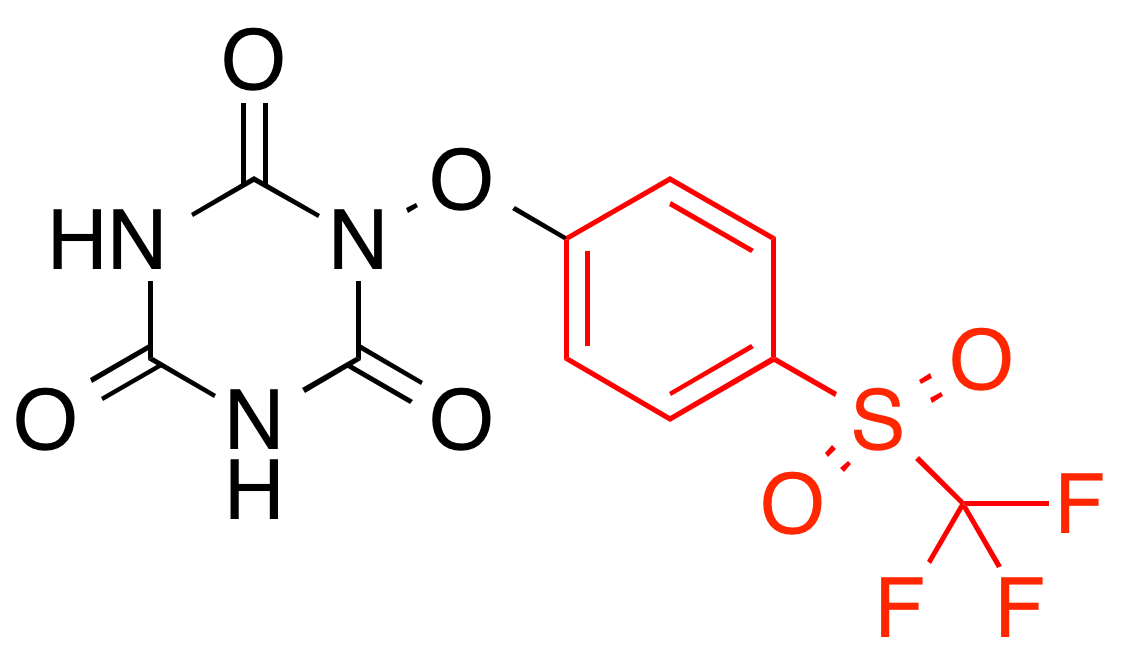
\includegraphics[width=3.3cm]{figures/jorge-figures/9.png}\\
\midrule
Fragments most activated by toxicity feature on NR-AHR dataset
%& \molfeaturetox{7}{14} & \molfeaturetox{7}{6} & \molfeaturetox{7}{5}
& 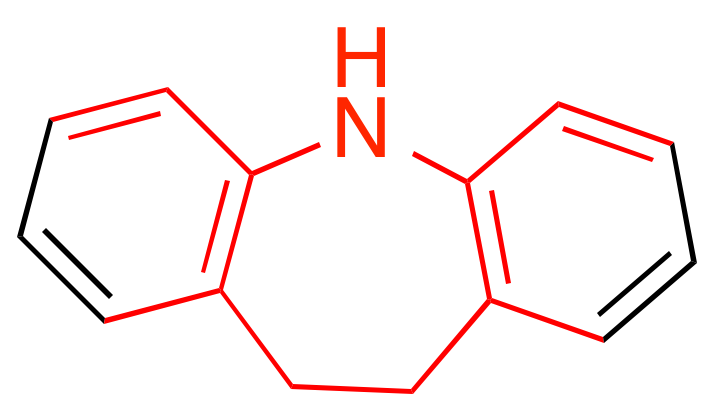
\includegraphics[width=2.2cm]{figures/jorge-figures/10.png} 
& 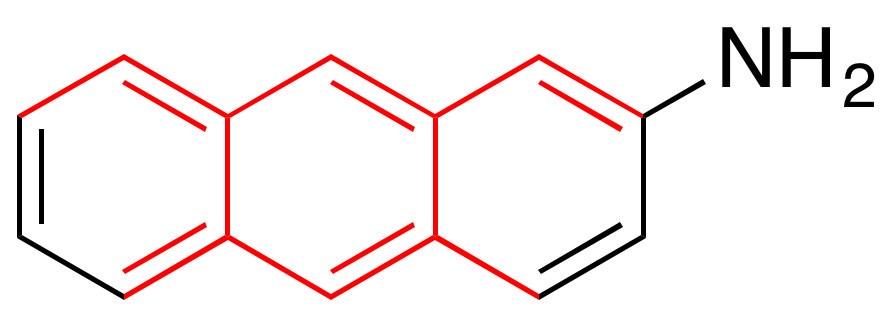
\includegraphics[width=3.3cm]{figures/jorge-figures/11.png}
& 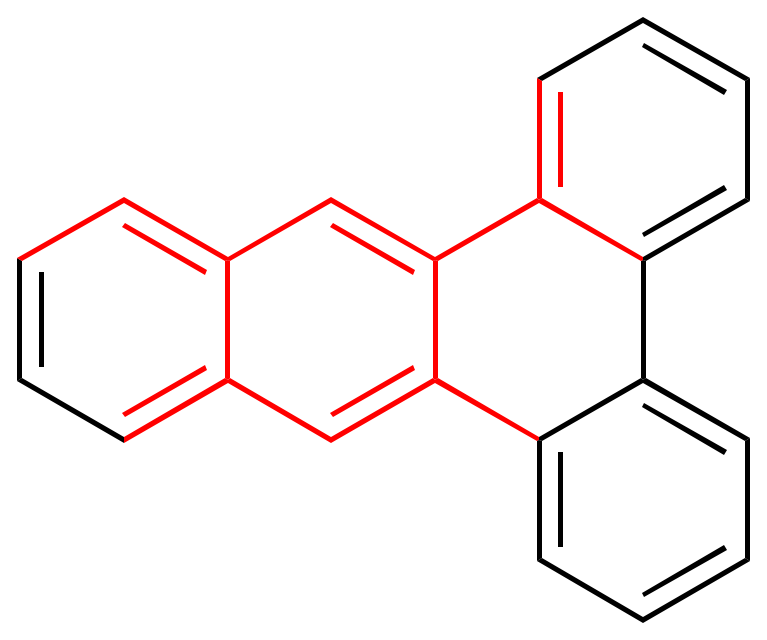
\includegraphics[width=2.9cm]{figures/jorge-figures/12.png}\\
\end{tabular}
\vspace{-3mm}
\caption{Visualizing fingerprints optimized for predicting toxicity.
Shown here are representative samples of molecular fragments (highlighted in red) which most activate each feature.
\emph{Top row:} the most predictive feature identifies groups containing a sulphur atom attached to an aromatic ring.
\emph{Bottom row:} the most predictive feature identifies fused aromatic rings, also known as polycyclic aromatic hydrocarbons, a known carcinogen.
}
\label{fig:learned features toxicity}
\end{figure}

\citet{unterthiner2015toxicity} constructed similar visualizations by searching for molecules that most activated neurons in a deep neural network on top of fixed circular fingerprints.
However, given fixed fingerprints, it's not clear how to automatically determine which fragments are relevant to the output.
\citet{unterthiner2015toxicity} did this in a semi-manual way: in order to determine which fragments of the molecules were predictive of toxicity, they searched over a list of substructures already known to be toxic (toxicophores) to find the toxic substructure that most correlated with the given neuron.
In contrast, our vizualizations are generated automatically, without the need to restrict the range of possible answers beforehand.

\subsection{Predictive Performance}

We ran several experiments to compare the predictive performance of neural fingerprints to that of the standard state-of-the-art setup:  circular fingerprints fed into a fully-connected neural network.

\paragraph{Experimental setup}
Our pipeline takes as input the SMILES~\citep{weininger1988smiles} string encoding of each molecule, which is then converted into a graph using RDKit~\citep{rdkit}.
We also used RDKit to produce the extended circular fingerprints used as the baseline.
Hydrogen atoms were treated implicitly.

In our convolutional networks, the initial atom and bond features were chosen to be similar to those used by ECFP:
Initial atom features concatenated a one-hot encoding of the element index, the degree, the number of attached hydrogen atoms, and the implicit valence, and an aromaticity indicator.
The bond features were a concatenation of whether the bond type was single, double, triple, or aromatic, whether the bond was conjugated, and whether the bond was part of a ring.

Training used batch normalization~\citep{ioffe2015batch}.
%Because batch normalization consistently led to better validation errors on both models, we eventually made it mandatory.
We also experimented with \texttt{tanh} vs \texttt{relu} activation functions for both the neural fingerprint net and the fully-connected nets.
\texttt{relu} had a slight but consistent performance advantage on the validation set.
We also experimented with dropconnect~\citep{wan2013regularization}, a variant of dropout in which weights are randomly set to zero instead of hidden units, but found that it led to worse validation error in general.

Each experiment optimized for 1000 minibatches of size 100 using the Adam algorithm~\citep{Adam14}, a variant of RMSprop that includes momentum.

\paragraph{Bayesian Optimization}
To optimize hyperparameters, we used Whetlab, a commercial implementation of Bayesian optimization~\citep{snoek2012practical}.
The hyperparameters of both methods were optimized using 200 trials for each experiment.
The following hyperparameters were optimized: log learning rate, log of Adam's $\beta_1$ and $\beta_2$ parameters, log of the initial weight scale, the log $L_2$ penalty, fingerprint length, fingerprint depth (up to 6), and the size of the hidden layer in the fully-connected network.
Additionally, the size of the hidden feature vector in the convolutional neural fingerprint networks was optimized.

\paragraph{Datasets}
We compared the performance of standard circular fingerprints against our neural fingerprints on a variety of domains:
%
\begin{itemize}
\item {\bf Solubility:} \cite{delaney_data_2004} measured the aqueous solubility of 1144 molecules.
\item{\bf Drug efficacy:} \citet{gamo2010thousands} measured the half maximal effective concentration (EC$_{50}$) {\it in vitro} of 20,000 molecules against a sulfide-resistant strain of {\it P. falciparum}.
\item {\bf Toxicity:} The \citet{tox21} released several assays measuring the toxicity of thousands of compounds.
We measured performance on the MMP stress response panel, whose predictive target was a binary response.
\item {\bf Organic photovoltaic efficiency:} The Harvard Clean Energy Project~\citet{hachmann2011harvard} has run millions of molecules through a DFT simulation to estimate the photovoltaic efficiency of organic molecules.
Each simulation requires several CPU hours, meaning that accurately predicting outcome of the simulation can greatly speed up the virtual screening process.
\end{itemize}
%
To examine the applicability of neural fingerprints to the relatively small size of datasets commonly encountered, we subsampled 1000 points from each dataset.

\paragraph{Predictive accuracy}
Results are summarized in Table~\ref{table:main results}.
%
\begin{table}
\begin{tabular}{lll|cc}
Predicted property              & Dataset                     & Metric & Circular        & Neural   \\
\midrule
Solubility (log Mol/L)          & \citet{delaney_data_2004}   &   RMSE & 1.04 $\pm$ 0.06 & \bf{0.72} $\pm$ 0.05 \\
Drug efficacy (EC$_{50}$ in nM) & \citet{gamo2010thousands}   &   RMSE & \bf{1.17} $\pm$ 0.12 & \bf{1.15} $\pm$ 0.16 \\
Toxicity (Binary)               & \citet{tox21}               &   NLL  & 0.65 $\pm$ 0.3  & \bf{0.32} $\pm$ 0.08 \\
Photovoltaic efficiency (\%)    & \citet{hachmann2011harvard} &  RMSE  & 1.96 $\pm$ 0.3  & \bf{1.68} $\pm$ 0.15
\end{tabular}
\label{table:main results}
\caption{Predictive accuracy of neural fingerprints compared to standard circular fingerprints.
For the binary classification task, we measures negative log predictive likelihood (NLL).}
\end{table}
%
In all experiments, the neural fingerprints match or substantially beat the accuracy of circular fingerprints.

\paragraph{Software}
Automatic differentiation (AD) software packages such as
Theano~\citep{Bastien-Theano-2012} significantly speed up development time by providing gradients automatically, but can only handle limited control structures and indexing.
Since we required relatively complex control flow and indexing in order to implement variants of Algorithm \ref{alg:neural}, we used a more flexible automatic differentiation package for Python, Autograd (\url{github.com/HIPS/autograd)}.
This package differentiates standard Numpy~\citep{oliphant2007python} code, and can differentiate code containing while loops, branches, and indexing.

Code for all experiments will be made available upon publication.

\section{Limitations}
%In this section we detail some limitations of the neural fingerprint architecture used in this paper.

\paragraph{Computational cost}
Neural fingerprints have the same asymptotic complexity in the number of atoms and the depth of the network as circular fingerprints, but have additional terms due to the matrix multiplies necessary to transform the feature vector at each step.
To be precise, computing the neural fingerprint of depth $R$, fingerprint length $L$ of a molecule with $N$ atoms using a molecular convolutional net having $F$ features at each layer costs $\mathcal{O}(RNFL + RNF^2)$.
In practice, training neural networks on top of circular fingerprints usually took several minutes, while training both the fingerprints and the network on top took on the order of an hour.

\paragraph{Limited computation at each layer}
How complicated should we make the function that goes from one layer of the network to the next?
In this paper we chose the simplest feasible architecture: a single layer of a neural network.
However, it may be fruitful to apply multiple layers of nonlinearities between each message-passing step (as in \cite{graphnn2009}), or to make information preservation easier by adapting the Long Short-Term Memory~\citep{hochreiter1997long} architecture to pass information upwards.

\paragraph{Limited information propagation across the graph}
The local message-passing architecture developed in this paper scales well in the size of the graph (due to the low degree of organic molecules), but its ability to propagate information across the graph is limited by the depth of the network.
This may be appropriate for small graphs such as those representing the small organic molecules used in this paper.
However, in the worst case, it can take a depth $\frac{N}{2}$ network to distinguish between graphs of size $N$.
To avoid this problem, \citet{bruna2013spectral} proposed a hierarchical clustering of graph substructures.
A tree-structured network could examine the structure of the entire graph using only $\log(N)$ layers, but would require learning to parse molecules.
Techniques from natural language processing~\citep{tai2015improved} might be fruitfully adapted to this domain.

\paragraph{Inability to distinguish stereoisomers}
Special bookkeeping is required to distinguish between stereoisomers, including enantomers (mirror images of molecules) or {\it cis/trans} isomers (rotation around double bonds).
Most circular fingerprint implementations have the option to make these distinctions.
Neural fingerprints could be extended to be sensitive to stereoisomers, but this remains for future work.

%\paragraph{Inapplicability to novel domains without retraining}
%Circular fingerprints have a useful property: their feature dimension is implicitly infinite.
%Because each possible substructure always maps to 

%\paragraph{Preserve asymmetries explicitly or implicitly}
%If we tie the weights of all neighboring vertices, then ordering information is lost locally, although it is still preserved implicitly in the relations between nodes in the next layer.

%\paragraph{3D features}
%How to extend this to using 3d features?

%\subsection{Interpretability}
%[Idea: Use nested dropout to allow a variable-sized descriptor.]
%Explain that it's analogous to PCA for neural nets


\section{Related work}
This work is similar in spirit to the Neural Turing Machine~\citep{graves2014neural}, in the sense that we take an existing discrete computational architecture, and make each part differentiable in order to do gradient-based optimization.

\paragraph{Convolutional neural networks}
Convolutional neural networks have been used to model images, speech, and time series~\citep{lecun1995convolutional}.
However, standard convolutional architectures use a fixed computational graph, making them difficult to apply to objects of varying size or structure, such as molecules.
More recently, \cite{KalchbrennerACL2014} and others have developed a convolutional neural network architecture for modeling sentences of varying length.

\paragraph{Neural fingerprints}
The most closely related work is \citet{lusci2013deep}, who build a neural network having graph-valued inputs.
Their approach is to remove all cycles and build the graph into a tree structure, choosing one atom to be the root.
A recursive neural network~\citep{socher2011dynamic, socher2011semi} is then run from the leaves to the root to produce a fixed-size representation.
Because a graph having $N$ nodes has $N$ possible roots, all $N$ possible graphs are constructed.
The final descriptor is a sum of the representations computed by all distinct graphs.
There are as many distinct graphs as there are atoms in the network.
The computational cost of this method thus grows as $\mathcal{O}(F^2N^2)$, where $F$ is the size of the feature vector and $N$ is the number of atoms, making it less suitable for large molecules.

\paragraph{Neural nets for quantitative structure-activity relationship (QSAR)}
The modern standard for predicting properties of novel molecules is to compose circular fingerprints with fully-connected neural networks or other regression methods.
\cite{dahl2014multi} used circular fingerprints as inputs to an ensemble of neural networks, Gaussian processes, and random forests.
\cite{ramsundar2015massively} used circular fingerprints (of depth 2) as inputs to a multitask neural network, showing that multiple tasks helped performance.

%\paragraph{Machine learning for identifying promising molecules}
%\cite{Eckert2007225, bergeron2011modeling} provide reviews of the field.
%\cite{tingley2014towards} used a variety of standard machine learning algorithms to predict the photovoltaic efficiency of organic molecules.

\paragraph{Neural networks on fixed graphs}
\cite{bruna2013spectral} introduce convolutional networks on graphs in the regime where the graph structure is fixed, and each training example differs only in having different features at the vertices of the same graph.
In contrast, our networks address the situation where each training input is a different graph.

\paragraph{Neural networks on input-dependent graphs}
\cite{graphnn2009} propose a neural network model for graphs having an interesting training procedure.
The forward pass consists of running a message-passing scheme to equilibrium, a fact which allows the reverse-mode gradient to be computed without storing the entire forward computation.
They apply their network to predicting mutagenesis of molecular compounds as well as web page rankings.
\cite{micheli2009neural} also propose a neural network model for graphs with a learning scheme whose inner loop optimizes not the training loss, but rather the correlation between each newly-proposed vector and the training error residual.
They apply their model to a dataset of boiling points of 150 molecular compounds.
Our paper builds on these ideas, with the following differences:
Our method replaces their complex training algorithms with simple gradient-based optimization, generalizes existing circular fingerprint computations, and applies these networks in the context of modern QSAR pipelines which use neural networks on top of the fingerprints to increase model capacity.

\paragraph{Unrolled inference algorithms}
\citet{hershey2014deep} and others have noted that iterative inference procedures sometimes resemble the feedforward computation of a recurrent neural network.
One natural extension of these ideas is to parameterize each inference step, and train a neural network to approximately match the output of exact inference using only a small number of iterations.
The neural fingerprint, when viewed in this light, resembles an unrolled message-passing algorithm on the original graph.


\section{Conclusion}
We generalized existing hand-crafted molecular features to allow their optimization for diverse tasks.
By making each operation in the the feature pipeline differentiable, we can use standard neural-network training methods to scalably optimize the parameters of these neural molecular fingerprints.
We examined the interpretability and predictive performance of these new fingerprints.

Data-driven features have already replaced hand-crafted features in speech recognition, machine vision, and natural-language processing.
Carrying out the same task for virtual screening seems like a natural next step.

%\section*{Acknowledgments}
\bibliography{references.bib}
\bibliographystyle{include/icml2015}
\end{document}